\documentclass[10pt,twoside,a4paper]{article}

%  EDIT THIS SECTION  %%%%%%%%%%%%%%%%%%%%%%%%%%%%%%%%%%%%%%%%%%%%%%%%%%%%%%%%%%%%%

\newcommand{\Title}{\textbf{A LaTeX template for Tektonika}} % Manuscript title goes here
\newcommand{\shortTitle}{LaTeX template} % Short title for header goes here
\newcommand{\FirstAuthor}{Firstauthor et al.\xspace} % First author goes here. Leave blank if opting for blind review.
\newcommand{\AllAuthors}{A. Firstauthor\textsuperscript{1}*, 
						 B. Second-Author\textsuperscript{2} \& 
						 C. Thirdauthor\textsuperscript{1,2}} % Author list goes here, with affiliations defined. Corresponding author email address is defined in the same way. Leave blank if opting for blind review.
\newcommand{\Year}{2022} % Year goes here
\newcommand{\Affiliation}{\textsuperscript{1}{Department of Geology, A University, Acity, UK}\\
						  \textsuperscript{2}{School of Earth Sciences,  Another University, Bcity, Norway}}
\newcommand{\CorrEmail}{{*}Corresponding author (e-mail: \url{afirstauthor@auniversity.ac.uk})}
\newcommand{\AbstractText}{\textbf{
Abstract text goes here. Max 250 words.}}
%%%%%%%%%%%%%%%%%%%%%%%%%%%%%%%%%%%%%%%%%%%%%%%%%%%%%%%%%%%%%%%%%%%%%%%%%%

%  DO NOT EDIT THIS SECTION  %%%%%%%%%%%%%%%%%%%%%%%%%%%%%%%%%%%%%%%%%%%%%%%%%%%%%%%%

% Font set up
\usepackage[default]{opensans}

% Page set up
%\usepackage[tmargin=1in,bmargin=1in,lmargin=0.9 in,rmargin=0.9in]{geometry} 
\usepackage[top=20mm,bottom=25mm,left=20mm,right=20mm,headheight=17pt,includefoot,heightrounded]{geometry} 
\renewcommand{\baselinestretch}{1.15}
\setlength{\columnsep}{7mm}
\usepackage{lastpage}


% Title and section set up
\usepackage{titlesec} 
\titleformat{\section}{\large \bfseries \raggedright}{\thesection}{2mm}{}
\titleformat{\subsection}{\bfseries \itshape \raggedright}{\thesubsection}{2mm}{}
\titleformat{\subsubsection}{\itshape \raggedright}{\thesubsubsection}{2mm}{}
\renewcommand{\thesubsubsection}{\emph{\thesubsection.\arabic{subsubsection}}}

% Author set up
\usepackage[affil-sl]{authblk} 
\setcounter{Maxaffil}{3}
\renewcommand\Affilfont{\itshape\small}
\renewcommand{\thefootnote}{\fnsymbol{footnote}}

% Hyperlink set up
\usepackage{xcolor} 
\definecolor{PUSblue}{HTML}{005FA8}
\usepackage{hyperref} 
\hypersetup{colorlinks = true, 
			citecolor = PUSblue,
			linkcolor=PUSblue,
			urlcolor  = PUSblue}
\urlstyle{same}

% Language set up
\usepackage{lipsum} 
\usepackage[pangram]{blindtext}
\usepackage{fancyhdr}
\usepackage[english]{babel}

% Math/Equation set up
\usepackage{sfmath} 
\usepackage{amsmath}
\usepackage{textgreek}
\usepackage[font=small,labelfont=bf]{caption}

% Figures and tables
\usepackage{graphicx} 
\usepackage{booktabs}
\usepackage{longtable}

% Bibliography
\usepackage[sectionbib,elide]{natbib}
\bibliographystyle{apalike}
\setlength{\bibsep}{0.0pt}


% Line numbers
\usepackage{lineno}
\linenumbers % Enable line numbers to facilitate review process (compile twice).

% Abstract
\usepackage{abstract}
\renewcommand{\abstractname}{}
\renewcommand{\abstractnamefont}{\normalfont \large \bfseries}

% Headers
\pagestyle{fancy}
\fancyhf{}
\fancyhead[LE]{\shortTitle}
\fancyhead[RE]{\sc \FirstAuthor, \ \Year}
\fancyhead[LO]{\journal, \vol}
\fancyhead[RO]{\doi}
%\rfoot{Page \thepage}
\rfoot{\thepage~of \pageref*{LastPage}}
\fancypagestyle{firststyle}
{
   \fancyhf{}
   \fancyhead{
\includegraphics[width=\textwidth]{article_banner.png}}
%   \renewcommand{\footrulewidth}{0.4pt}
   \rfoot{\thepage~of \pageref*{LastPage}}
%   \lfoot{\small{\journal, \vol\\\doi\\}}
%   \cfoot{\setlength{\parindent}{5cm}{\small{\raggedright{\dSubmitted\\\dAccepted\\\dOnline}}}}

}

% Document elements
\title{%\normalsize\Head\\
\vspace{5mm}
\LARGE\Title}
\author{\AllAuthors
~\\\Affiliation
\\\CorrEmail}

\begin{document}
\date{}


\maketitle
\thispagestyle{firststyle}

\begin{abstract}\normalsize
\AbstractText
\end{abstract}

\vspace{5mm}
\vspace{5mm}


%%%%%%%%%%%%%%%%%%%%%%%%%%%%%%%%%%%%%%%%%%%%%%%%%%%%%%%%%%%%%%%%%%%%%%%%%%

%  EDIT THIS SECTION  %%%%%%%%%%%%%%%%%%%%%%%%%%%%%%%%%%%%%%%%%%%%%%%%%%%%%%%%%%%%%

\section{Introduction}
The main body of the text should go here.

\subsection{Subsections appear like this}
Figure sizes should not exceed 85x200 mm for single column figures or 175x200 mm for two column figures.

\begin{figure}[h!]\centering
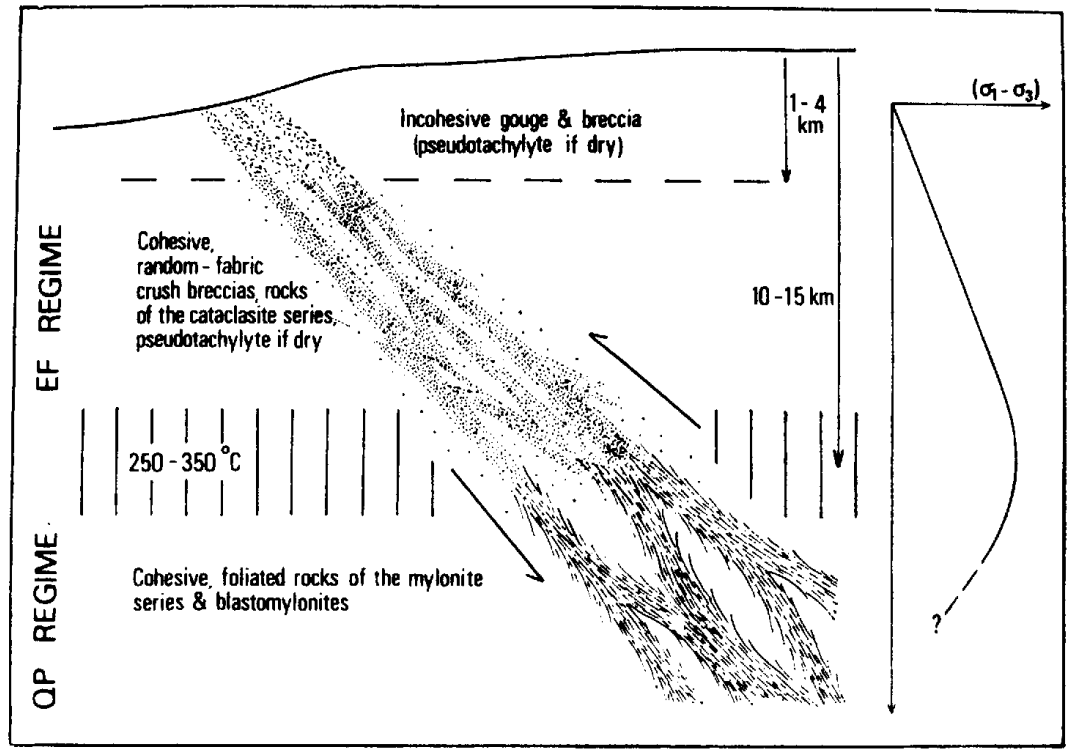
\includegraphics[width=0.5\textwidth]{SibsonFZ.png} 
\caption{Conceptual model of a major fault zone.}
\label{fig:1}
\end{figure}

\subsubsection{Sub-subsections appear like this}

Equations are defined in the \{equation\} environment:
 \begin{equation}
\dot{\varepsilon} = A\sigma^{n} f_{H_{2}O}^{r} e^{({\frac{-Q}{RT}})}
\end{equation}


\section{More sections}
Citations may either be inline \citet{sibson1977fault} or in parentheses \citep{sibson1977fault}.

\section*{Acknowledgements} % Please upload separately if opting for blind review.
Thank all relevant parties and acknowledge funding sources, if any.
\section*{Author contributions} % Please upload separately if opting for blind review.
Tell us who did what.
\section*{Data availability}
Authors should direct readers to an open access repository such as figshare or Github, where data are made available.
\bibliography{mybibfile} % a separate bibfile is required. Please upload this file along with the compiled manuscript and source file.

%%%%%%%%%%%%%%%%%%%%%%%%%%%%%%%%%%%%%%%%%%%%%%%%%%%%%%%%%%%%%%%%%%%%%%%%%%
\end{document}
